\chapter{Simetria e grupos pontuais}\label{ch:b3:point-groups}

Gire um floco de neve de sessenta graus e nada muda; gire uma molécula de
benzeno do mesmo ângulo, e seus seis carbonos e seis hidrogênios caem
exatamente uns nos lugares dos outros. A simetria de uma molécula decide
várias de suas propriedades antes de qualquer cálculo: se ela pode ter um
momento dipolar, se pode existir em duas formas especulares, quais de suas
vibrações absorvem luz infravermelha, quais orbitais podem se misturar. Para
usá-la, os químicos tomaram emprestada da matemática a linguagem dos grupos.
Este capítulo define as \omterm{def:b3:point-groups:operation}{operações de simetria} de uma molécula, reúne-as em
seu \omterm{def:b3:point-groups:point-group}{grupo pontual}, dá um procedimento para encontrar esse grupo, demonstra
dois teoremas sobre polaridade e quiralidade e apresenta as \omterm{def:b3:point-groups:irrep}{tabelas de
caracteres} sobre as quais se constrói o \cref{ch:b3:group-theory-applied}.

\begin{recall}
O volume do 1.º ano previu as formas moleculares com o modelo VSEPR, definiu
o momento dipolar de uma molécula polar e definiu a quiralidade: uma molécula
quiral não pode ser sobreposta à sua imagem especular. O volume do 2.º ano
usou a simetria, em palavras, para construir os orbitais de fragmento de
\ce{H2O} e de \ce{NH3}.
\end{recall}

\begin{omfigure}
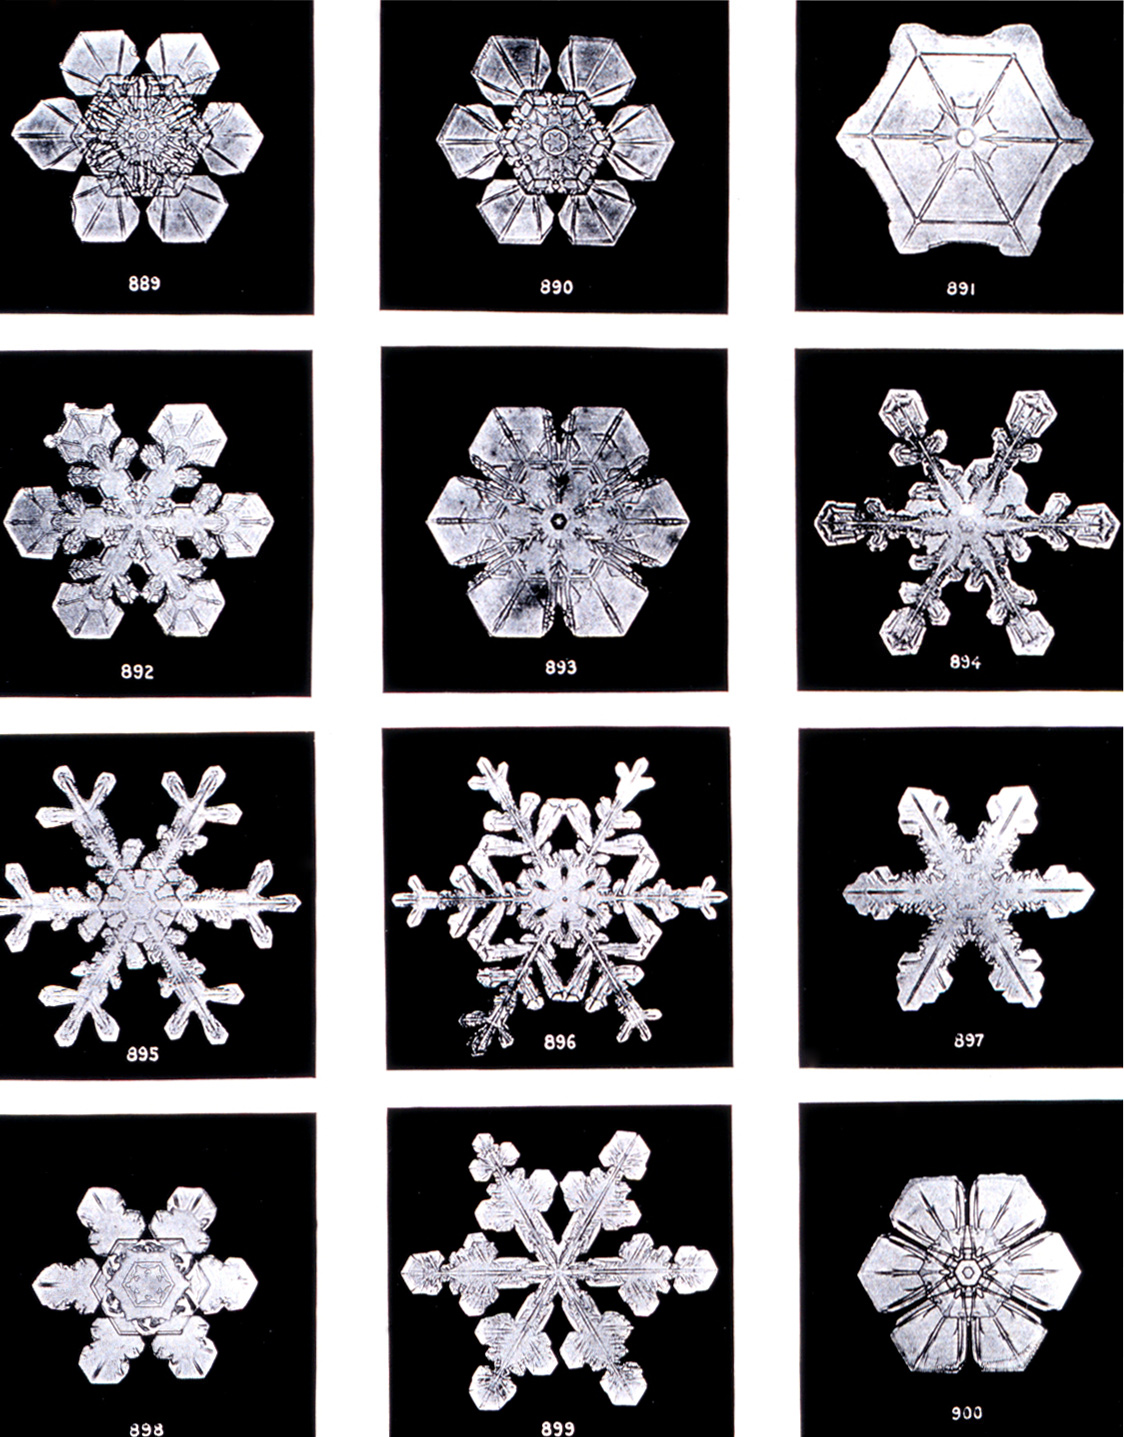
\includegraphics[width=0.4\linewidth]{images/book4/bentley-snowflakes.jpg}\hspace{1em}%
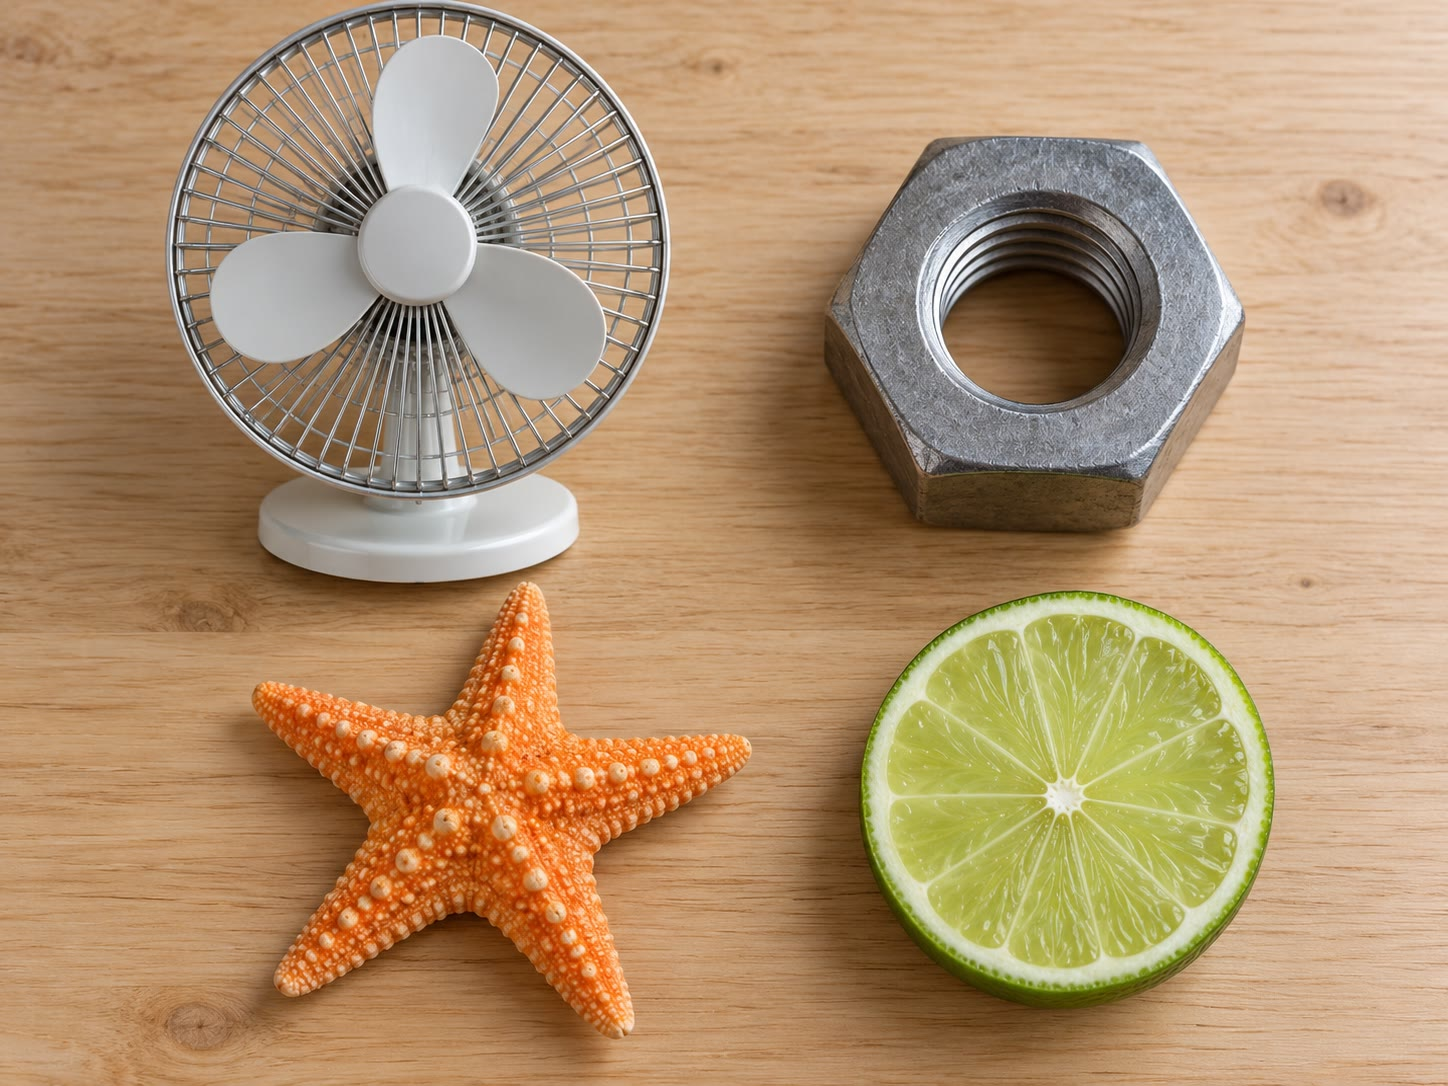
\includegraphics[width=0.48\linewidth]{images/book4/ai/b3-04-symmetric-objects.jpg}

{\small À esquerda: cristais de neve fotografados por Wilson Bentley por volta
de 1902, cada um com simetria de ordem seis. À direita: objetos do cotidiano
com simetria de rotação de ordem três, seis e cinco.}
\end{omfigure}

\section{Operações e elementos de simetria}

\begin{definition}[Operação de simetria, elemento de simetria]\label{def:b3:point-groups:operation}
Uma \emph{operação de simetria}\index{operacao de simetria@operação de simetria} é um movimento ou
uma reflexão que deixa uma molécula em uma configuração indistinguível da
original (cada átomo em uma posição ocupada antes por um átomo da mesma
espécie). Um \emph{elemento de simetria}\index{elemento de simetria} é o objeto
geométrico --- um ponto, uma reta, um plano --- em relação ao qual a
operação é efetuada.
\end{definition}

Toda molécula tem a operação identidade $E$, que não faz nada. As
demais são de quatro tipos.

\begin{definition}[Eixo de rotação própria, eixo principal]\label{def:b3:point-groups:rotation}
Um \emph{eixo de rotação própria}\index{eixo de rotacao propria@eixo de rotação própria} $C_n$ é uma reta
em torno da qual uma rotação de $2\pi/n$ é uma \omterm{def:b3:point-groups:operation}{operação de simetria}, também
escrita $C_n$; suas potências $C_n^k$ são rotações de $2\pi k/n$, e $C_n^n = E$. O
eixo de maior $n$ é o \emph{eixo principal}\index{eixo principal}, tomado
como $z$.
\end{definition}

\begin{definition}[Planos especulares]\label{def:b3:point-groups:mirror}
Um \emph{plano especular}\index{plano especular} $\sigma$ é um plano em relação ao qual
a reflexão é uma \omterm{def:b3:point-groups:operation}{operação de simetria}; $\sigma^2 = E$. Um plano especular é um
\emph{plano especular vertical}\index{plano especular vertical} $\sigma_v$ se
contém o \omterm{def:b3:point-groups:rotation}{eixo principal}, um \emph{plano especular
horizontal}\index{plano especular horizontal} $\sigma_h$ se é perpendicular a
ele, e um \emph{plano especular diedral}\index{plano especular diedral}
$\sigma_d$ se contém o \omterm{def:b3:point-groups:rotation}{eixo principal} e divide ao meio o ângulo entre
dois eixos $C_2$ perpendiculares a ele.
\end{definition}

\begin{definition}[Centro de inversão]\label{def:b3:point-groups:inversion}
Um \emph{centro de inversão}\index{centro de inversao@centro de inversão} $i$ é um ponto
em relação ao qual a inversão, $(x, y, z) \mapsto (-x, -y, -z)$, é uma \omterm{def:b3:point-groups:operation}{operação de
simetria}.
\end{definition}

\begin{definition}[Eixo de rotação imprópria]\label{def:b3:point-groups:improper}
Um \emph{eixo de rotação imprópria}\index{eixo de rotacao impropria@eixo de rotação imprópria} $S_n$ é uma
reta em torno da qual uma rotação de $2\pi/n$ seguida de uma reflexão no plano
perpendicular a ela é uma \omterm{def:b3:point-groups:operation}{operação de simetria}. $S_1 = \sigma$ e $S_2 = i$.
\end{definition}

\begin{example}[Elementos de quatro moléculas]\label{ex:b3:point-groups:elements}
\ce{H2O}: $E$, um eixo $C_2$ que divide ao meio o ângulo H--O--H e dois planos
verticais, o plano molecular e o plano perpendicular a ele. \ce{NH3}:
$E$, um $C_3$ passando por N (operações $C_3$ e $C_3^2$) e três $\sigma_v$, cada
um contendo uma ligação N--H. \ce{BF3}: um $C_3$, três $C_2$ ao longo das ligações B--F,
$\sigma_h$ (o plano molecular), três $\sigma_v$ e um $S_3$. \ce{CH4}: quatro
$C_3$ ao longo das ligações C--H, três $C_2$ que dividem ao meio ângulos H--C--H,
que são também eixos $S_4$, e seis $\sigma_d$, cada um contendo duas ligações C--H
(figura abaixo).
\end{example}

\begin{omfigure}
\begin{tikzpicture}[font=\small]
  % H2O, side view: molecular plane xz (shaded), C2 along z
  \begin{scope}
    \fill[omDef!10] (-1.5,-1.0) -- (1.5,-1.0) -- (1.5,1.2) -- (-1.5,1.2) -- cycle;
    \fill[omThm!12, opacity=0.8] (-0.45,-1.35) -- (0.45,-0.65) -- (0.45,1.55) -- (-0.45,0.85) -- cycle;
    \draw[densely dashed, black!70] (0,-1.4) -- (0,1.7) node[above] {$C_2$};
    \node[aO] (o) at (0,0.5) {};
    \node[aH] (h1) at (-0.95,-0.25) {};
    \node[aH] (h2) at (0.95,-0.25) {};
    \begin{scope}[on background layer]
      \draw[bond] (o.center) -- (h1.center) (o.center) -- (h2.center);
    \end{scope}
    \node[omDef, anchor=north west] at (-1.5,1.2) {$\sigma_v(xz)$};
    \node[omThm, anchor=west] at (0.5,-0.85) {$\sigma_v'(yz)$};
    \node[anchor=north] at (0,-1.6) {\ce{H2O}, $C_{2v}$};
  \end{scope}
  % NH3, top view along C3
  \begin{scope}[xshift=4.0cm]
    \foreach \a in {90,210,330}{\draw[ommirror] (0,0) -- (\a:1.35); \draw[ommirror, black!40] (0,0) -- (\a+180:1.0);}
    \foreach \a in {90,210,330}{\node[aH] at (\a:0.95) {};}
    \node[aN] at (0,0) {};
    \pic at (0,0) {omthreefold};
    \node[anchor=north] at (0,-1.6) {\ce{NH3}, $C_{3v}$ (de cima)};
  \end{scope}
  % BF3, top view; sigma_h = plane of the paper (thick circle)
  \begin{scope}[xshift=8.0cm]
    \draw[ommirror] (0,0) circle (1.3);
    \foreach \a in {90,210,330}{\draw[ommirror] (\a:1.3) -- (\a+180:1.3);}
    \foreach \a in {90,210,330}{\pic[rotate=\a-90] at (\a:1.42) {omtwofold}; \pic[rotate=\a-90] at (\a+180:1.42) {omtwofold};}
    \foreach \a in {90,210,330}{\node[aF] at (\a:0.95) {};}
    \node[aX={pink!70!gray}{5.6mm}] at (0,0) {};
    \pic at (0,0) {omthreefold};
    \node[anchor=north] at (0,-1.6) {\ce{BF3}, $D_{3h}$ (de cima)};
  \end{scope}
\end{tikzpicture}

{\small \omterm{def:b3:point-groups:operation}{Elementos de simetria}. \ce{H2O}: o eixo $C_2$ (tracejado) e dois \omterm{def:b3:point-groups:mirror}{planos
especulares verticais}. \ce{NH3} e \ce{BF3} vistos ao longo de seu \omterm{def:b3:point-groups:rotation}{eixo principal}
(símbolo triangular): os traços grossos são \omterm{def:b3:point-groups:mirror}{planos especulares} vistos de perfil;
em \ce{BF3}, o círculo grosso marca o \omterm{def:b3:point-groups:mirror}{plano especular horizontal} (o plano da
página) e os símbolos em lente, os três eixos $C_2$ contidos nele.}
\end{omfigure}

\section{Grupos}

\begin{proposition}[Produtos de operações de simetria]\label{prop:b3:point-groups:closure}
Efetuar sucessivamente duas \omterm{def:b3:point-groups:operation}{operações de simetria} de uma molécula dá ainda
uma \omterm{def:b3:point-groups:operation}{operação de simetria} dessa molécula. Com $E$ e o inverso de cada
operação, o conjunto das \omterm{def:b3:point-groups:operation}{operações de simetria} é um grupo: um produto
associativo, um elemento neutro, um inverso para cada elemento.
\end{proposition}

\begin{proof}
Cada operação deixa a molécula indistinguível de si mesma, logo duas
sucessivas também. O produto de operações (composição de transformações do
espaço) é associativo; $E$ é o elemento neutro; uma operação desfeita (uma
rotação do ângulo oposto, uma reflexão repetida) é também uma \omterm{def:b3:point-groups:operation}{operação de simetria}.
\end{proof}

\begin{proposition}[Um ponto comum]\label{prop:b3:point-groups:fixed-point}
Todos os \omterm{def:b3:point-groups:operation}{elementos de simetria} de uma molécula finita passam por um mesmo ponto.
\end{proposition}

\begin{proof}
Toda \omterm{def:b3:point-groups:operation}{operação de simetria} leva cada átomo sobre um átomo de mesma massa,
logo deixa o centro de massa inalterado. Uma rotação fixa apenas os pontos de
seu eixo, uma reflexão os de seu plano, uma rotação imprópria ou uma inversão
um único ponto: todo elemento contém o centro de massa.
\end{proof}

\begin{definition}[Grupo pontual, ordem de um grupo pontual]\label{def:b3:point-groups:point-group}
O grupo de todas as \omterm{def:b3:point-groups:operation}{operações de simetria} de uma molécula é seu \emph{grupo
pontual}\index{grupo pontual}, assim chamado porque um ponto permanece fixo. O
número de suas operações é a \emph{ordem de um grupo pontual}\index{ordem de um grupo pontual},
$h$.
\end{definition}

\begin{example}[O grupo da água]\label{ex:b3:point-groups:c2v}
As quatro operações $E$, $C_2$, $\sigma_v(xz)$, $\sigma_v'(yz)$ de \ce{H2O} formam um
grupo de ordem 4. Sua tábua de multiplicação (a operação da linha efetuada
depois da operação da coluna) é
\begin{center}\small
\begin{tabular}{c|cccc}
\hline
 & $E$ & $C_2$ & $\sigma_v(xz)$ & $\sigma_v'(yz)$\\ \hline
$E$ & $E$ & $C_2$ & $\sigma_v(xz)$ & $\sigma_v'(yz)$\\
$C_2$ & $C_2$ & $E$ & $\sigma_v'(yz)$ & $\sigma_v(xz)$\\
$\sigma_v(xz)$ & $\sigma_v(xz)$ & $\sigma_v'(yz)$ & $E$ & $C_2$\\
$\sigma_v'(yz)$ & $\sigma_v'(yz)$ & $\sigma_v(xz)$ & $C_2$ & $E$\\ \hline
\end{tabular}
\end{center}
Por exemplo, um ponto $(x, y, z)$ refletido em $xz$ vai para $(x, -y, z)$ e,
girado de $\pi$ em torno de $z$, para $(-x, y, z)$: o mesmo que uma única
reflexão em $yz$.
\end{example}

\begin{definition}[Classe de operações de simetria, subgrupo]\label{def:b3:point-groups:class}
Duas operações $A$ e $B$ pertencem à mesma \emph{classe de operações de
simetria}\index{classe de operacoes de simetria@classe de operações de simetria} se $B = X^{-1}AX$ para alguma
operação $X$ do grupo: são o mesmo tipo de operação, visto em um referencial
deslocado por $X$. Um subconjunto de um grupo que é ele próprio um grupo é um
\emph{subgrupo}\index{subgrupo}; sua ordem divide a ordem do grupo.
\end{definition}

\begin{example}[Classes de \ce{NH3}]\label{ex:b3:point-groups:classes}
Em $C_{3v}$ ($h = 6$), as três reflexões formam uma classe (uma rotação $C_3$
leva cada plano em outro), as duas rotações $C_3$ e $C_3^2$ outra,
e $E$ forma sozinha uma classe: três classes, escritas $E$, $2C_3$, $3\sigma_v$. Em
$C_{2v}$, cada operação é sua própria classe: nenhuma operação transforma um
plano no outro.
\end{example}

\begin{definition}[Símbolo de Schoenflies]\label{def:b3:point-groups:schoenflies}
Um \omterm{def:b3:point-groups:point-group}{grupo pontual} é designado por seu \emph{símbolo de Schoenflies}\index{simbolo de Schoenflies@símbolo de Schoenflies}:
$C_n$ (um eixo $C_n$), $C_{nv}$ (acrescentando $n$ planos verticais), $C_{nh}$
(acrescentando $\sigma_h$), $D_n$ (acrescentando $n$ eixos $C_2$ perpendiculares a $C_n$), $D_{nh}$
e $D_{nd}$ (acrescentando $\sigma_h$, ou $n$ planos diedrais, a $D_n$), $S_{2n}$, os
grupos cúbicos $T_d$, $O_h$, $I_h$ do tetraedro, do octaedro e do
icosaedro, e $C_s$, $C_i$, $C_1$ para as moléculas que têm apenas um \omterm{def:b3:point-groups:mirror}{plano especular},
apenas um \omterm{def:b3:point-groups:inversion}{centro de inversão} ou nada. As moléculas lineares pertencem a
$C_{\infty v}$ ou a $D_{\infty h}$.
\end{definition}

\section{Atribuir um grupo pontual}

\begin{method}[Encontrar o grupo pontual de uma molécula]\label{met:b3:point-groups:assign}
\begin{enumerate}
  \item A molécula é linear? Com \omterm{def:b3:point-groups:inversion}{centro de inversão}, $D_{\infty h}$
        (\ce{CO2}, \ce{N2}); sem, $C_{\infty v}$ (\ce{HCl}, \ce{HCN}).
  \item Ela tem vários eixos de ordem alta ($n \ge 3$)? Forma tetraédrica:
        $T_d$; octaédrica: $O_h$; icosaédrica: $I_h$.
  \item Encontre o \omterm{def:b3:point-groups:rotation}{eixo principal} $C_n$ (nenhum: $C_s$ se há um plano, $C_i$ se há um
        centro, $C_1$ caso contrário).
  \item Há $n$ eixos $C_2$ perpendiculares a $C_n$? Se sim, o grupo é
        $D_{nh}$ (com $\sigma_h$), senão $D_{nd}$ (com $n$ $\sigma_d$), senão
        $D_n$.
  \item Se não: $C_{nh}$ (com $\sigma_h$), $C_{nv}$ (com $n$ $\sigma_v$), $S_{2n}$
        (apenas com um $S_{2n}$ colinear a $C_n$), senão $C_n$.
\end{enumerate}
\end{method}

\begin{omfigure}
\begin{tikzpicture}[font=\footnotesize, node distance=6mm and 11mm,
  q/.style={draw=black!60, fill=omDef!6, rounded corners=2pt, align=center, inner sep=3pt},
  g/.style={draw=black!60, fill=omProp!10, rounded corners=2pt, inner sep=3pt}]
  \node[q] (lin) {linear?};
  \node[g, right=of lin] (dinf) {$D_{\infty h}$ / $C_{\infty v}$ (com / sem $i$)};
  \node[q, below=of lin] (cub) {dois ou mais $C_n$, $n \ge 3$?};
  \node[g, right=of cub] (td) {$T_d$, $O_h$, $I_h$};
  \node[q, below=of cub] (cn) {um eixo $C_n$?};
  \node[g, right=of cn] (low) {$C_s$, $C_i$ ou $C_1$ (não)};
  \node[q, below=of cn] (c2) {$n$ $C_2 \perp C_n$?};
  \node[q, right=of c2, xshift=6mm] (dh) {$\sigma_h$?\; senão $n$ $\sigma_d$?};
  \node[g, right=of dh] (dg) {$D_{nh}$ / $D_{nd}$ / $D_n$};
  \node[q, below=of c2] (sh) {$\sigma_h$?\; senão $n$ $\sigma_v$?\; senão $S_{2n}$?};
  \node[g, right=of sh] (cg) {$C_{nh}$ / $C_{nv}$ / $S_{2n}$ / $C_n$};
  \draw[->] (lin) -- node[above] {sim} (dinf);
  \draw[->] (lin) -- node[left] {não} (cub);
  \draw[->] (cub) -- node[above] {sim} (td);
  \draw[->] (cub) -- node[left] {não} (cn);
  \draw[->] (cn) -- node[above] {não} (low);
  \draw[->] (cn) -- node[left] {sim} (c2);
  \draw[->] (c2) -- node[above] {sim} (dh);
  \draw[->] (dh) -- (dg);
  \draw[->] (c2) -- node[left] {não} (sh);
  \draw[->] (sh) -- (cg);
\end{tikzpicture}

{\small A busca de um \omterm{def:b3:point-groups:point-group}{grupo pontual}, na ordem do método.}
\end{omfigure}

\begin{example}[Uma galeria]\label{ex:b3:point-groups:gallery}
\ce{H2O}, \ce{CH2Cl2}, \ce{SO2}: $C_{2v}$. \ce{NH3}, \ce{CHCl3}: $C_{3v}$. \ce{BF3},
\ce{PCl5}: $D_{3h}$. \ce{CH4}, \ce{CCl4}: $T_d$. \ce{SF6}: $O_h$. Benzeno: $D_{6h}$.
Eteno: $D_{2h}$. Etano: $D_{3d}$ alternado, $D_{3h}$ eclipsado. Aleno
\ce{H2C=C=CH2}: $D_{2d}$, com os dois planos \ce{CH2} em ângulo reto. Ciclo-hexano
em cadeira: $D_{3d}$. trans-\ce{N2F2}: $C_{2h}$. \ce{CHFClBr}: $C_1$.
\end{example}

\begin{omfigure}
\tdplotsetmaincoords{60}{100}
\begin{tikzpicture}[tdplot_main_coords, scale=1.6, font=\small]
  \pic[transform shape] {omcubeo={2}};
  % depth order for view 60/100 (smallest first): H(0,0,0), H(0,2,2), C, H(2,2,0), H(2,0,2)
  \draw[densely dashed, omThm, thick] (-0.4,-0.4,-0.4) -- (2.5,2.5,2.5) node[anchor=south west] {$C_3$};
  \draw[densely dashed, omDef, thick] (1,1,-0.5) -- (1,1,2.6) node[anchor=south] {$S_4$, $C_2$};
  \node[aH] (h1) at (0,0,0) {};
  \node[aH] (h4) at (0,2,2) {};
  \node[aC] (c) at (1,1,1) {};
  \node[aH] (h2) at (2,2,0) {};
  \node[aH] (h3) at (2,0,2) {};
  \begin{scope}[on background layer]
    \draw[bond] (c.center) -- (h1.center) (c.center) -- (h2.center)
                (c.center) -- (h3.center) (c.center) -- (h4.center);
  \end{scope}
\end{tikzpicture}

{\small O metano em um cubo, com o carbono no centro e os hidrogênios em
vértices alternados. Uma diagonal do cubo que passa por um hidrogênio é um
eixo $C_3$ (há quatro); o eixo que passa pelos centros de duas faces opostas é
um eixo $C_2$ e $S_4$ (há três). O \omterm{def:b3:point-groups:point-group}{grupo pontual} é $T_d$, de ordem 24.}
\end{omfigure}

\section{Consequências: polaridade e quiralidade}

\begin{theorem}[Moléculas polares]\label{thm:b3:point-groups:polar}
Uma molécula só pode ter um momento dipolar permanente se seu \omterm{def:b3:point-groups:point-group}{grupo pontual}
for $C_1$, $C_s$, $C_n$ ou $C_{nv}$; o dipolo fica então ao longo do \omterm{def:b3:point-groups:rotation}{eixo principal}
(no plano, para $C_s$).
\end{theorem}

\begin{proof}
O momento dipolar é uma propriedade vetorial da molécula, logo toda \omterm{def:b3:point-groups:operation}{operação
de simetria} deve deixá-lo inalterado. Uma rotação em torno de um eixo deixa
inalterados apenas os vetores ao longo desse eixo; dois eixos não deixam
nenhum vetor não nulo; um $\sigma_h$, um $i$ ou um $S_n$ invertem todo vetor ao
longo do eixo; um $\sigma_v$ conserva os vetores contidos em seu plano. Um
dipolo não nulo exige, portanto, no máximo um eixo, nenhum $\sigma_h$, nenhum $i$,
nenhum $S_n$: os grupos listados.
\end{proof}

\begin{example}[Polar ou não]\label{ex:b3:point-groups:polar}
\ce{H2O}, \ce{NH3}, \ce{CHCl3} e \ce{SO2} ($C_{2v}$, $C_{3v}$) podem ser polares, e
são. \ce{BF3} ($D_{3h}$), \ce{CO2} ($D_{\infty h}$), \ce{CH4} ($T_d$), \ce{SF6} ($O_h$)
e trans-\ce{N2F2} ($C_{2h}$) não podem, quaisquer que sejam suas ligações polares.
\end{example}

\begin{theorem}[Moléculas quirais]\label{thm:b3:point-groups:chiral}
Uma molécula é quiral se, e somente se, não tem nenhum \omterm{def:b3:point-groups:improper}{eixo de rotação imprópria} $S_n$
(incluindo $S_1 = \sigma$ e $S_2 = i$).
\end{theorem}

\begin{proof}
Se a molécula tem um $S_n$, então $S_n = \sigma_hC_n$: a imagem especular $\sigma_h$
da molécula é igual a $C_n^{-1}$ aplicado à molécula depois de $S_n$, isto é,
à molécula girada --- sobreponível, logo aquiral. Reciprocamente, se a
molécula é aquiral, sua imagem especular $\sigma M$ pode ser levada sobre $M$ por um
movimento próprio $R$ (uma rotação em torno do centro de massa): $R\sigma$ é então uma
\omterm{def:b3:point-groups:operation}{operação de simetria}. Ela é imprópria (troca a quiralidade, sua matriz tem
determinante $-1$), e toda operação imprópria de um \omterm{def:b3:point-groups:point-group}{grupo pontual} é um
$S_n$ para algum $n$ (uma rotação seguida de uma reflexão no plano
perpendicular). Logo a molécula tem um $S_n$.
\end{proof}

\begin{example}[Uma molécula aquiral sem plano]\label{ex:b3:point-groups:s4}
Algumas moléculas não têm nem \omterm{def:b3:point-groups:mirror}{plano especular} nem \omterm{def:b3:point-groups:inversion}{centro de inversão} e, no
entanto, são aquirais graças a um eixo $S_4$: o caso clássico é um composto
espiro formado por dois anéis substituídos de modo idêntico, em ângulo reto,
de \omterm{def:b3:point-groups:point-group}{grupo pontual} $S_4$. A quiralidade não pode ser julgada procurando apenas um plano.
\end{example}

\section{Representações e tabelas de caracteres}

Cada \omterm{def:b3:point-groups:operation}{operação de simetria} move um ponto $(x, y, z)$ de modo linear: ela pode ser
escrita como uma matriz $3\times3$.

\begin{definition}[Representação matricial, caráter]\label{def:b3:point-groups:representation}
Uma \emph{representação matricial}\index{representacao matricial@representação matricial} $\Gamma$ de um
\omterm{def:b3:point-groups:point-group}{grupo pontual} associa a cada operação $R$ uma matriz quadrada $D(R)$ tal que
$D(R_1R_2) = D(R_1)D(R_2)$: os produtos de operações tornam-se produtos de
matrizes. O \emph{caráter}\index{carater@caráter} $\chi(R)$ de $R$ em $\Gamma$ é
o traço de $D(R)$.
\end{definition}

\begin{example}[As coordenadas em $C_{3v}$]\label{ex:b3:point-groups:xyz}
Para $C_3$ em torno de $z$, $D = \begin{psmallmatrix}\cos120^\circ & -\sin120^\circ &
0\\ \sin120^\circ & \cos120^\circ & 0\\ 0 & 0 & 1\end{psmallmatrix}$, de traço
$2\cos120^\circ + 1 = 0$; para $\sigma_v(xz)$, $D = \mathrm{diag}(1, -1, 1)$, traço
1; para $E$, traço 3. Os \omterm{def:b3:point-groups:representation}{caracteres} dessa representação são $(3, 0, 1)$ nas
classes $(E, 2C_3, 3\sigma_v)$. Todas as matrizes são diagonais por blocos, um
bloco $2\times2$ para $(x, y)$ e um bloco $1\times1$ para $z$: a
representação se decompõe em duas menores.
\end{example}

\begin{proposition}[Os caracteres são funções de classe]\label{prop:b3:point-groups:class-characters}
Operações da mesma classe têm o mesmo \omterm{def:b3:point-groups:representation}{caráter} em qualquer representação.
\end{proposition}

\begin{proof}
Se $B = X^{-1}AX$, então $D(B) = D(X)^{-1}D(A)D(X)$, e o traço não muda por
essa mudança de base: $\mathrm{tr}(P^{-1}MP) = \mathrm{tr}(M)$.
\end{proof}

\begin{proposition}[Redução por blocos]\label{prop:b3:point-groups:direct-sum}
Se uma base pode ser dividida em subconjuntos que cada operação leva em si
mesmos, todas as matrizes são diagonais por blocos, e a representação é a
soma das representações menores carregadas pelos subconjuntos; seus
\omterm{def:b3:point-groups:representation}{caracteres} são as somas dos \omterm{def:b3:point-groups:representation}{caracteres} destas.
\end{proposition}

\begin{proof}
Uma operação que leva cada subconjunto em si mesmo não tem elementos de
matriz entre subconjuntos diferentes; o traço de uma matriz diagonal por
blocos é a soma dos traços de seus blocos.
\end{proof}

\begin{definition}[Representação irredutível, tabela de caracteres, símbolo de Mulliken]\label{def:b3:point-groups:irrep}
Uma representação que não pode mais ser decomposta por nenhuma mudança de base é
uma \emph{representação irredutível}\index{representacao irredutivel@representação irredutível}. A
\emph{tabela de caracteres}\index{tabela de caracteres} de um \omterm{def:b3:point-groups:point-group}{grupo pontual} lista os
\omterm{def:b3:point-groups:representation}{caracteres} de suas representações irredutíveis, uma por linha, em suas classes,
uma por coluna, com as funções cartesianas e as rotações que se transformam
como cada linha. As linhas são designadas por seu \emph{símbolo de
Mulliken}\index{simbolo de Mulliken@símbolo de Mulliken}: $A$ ou $B$ para dimensão um (simétrica ou
antissimétrica sob a rotação principal), $E$ para dois, $T$ para três;
índices 1, 2 (simétrica ou antissimétrica sob um $C_2$ ou um $\sigma_v$), $g$, $u$
(sob a inversão), linhas (sob $\sigma_h$).
\end{definition}

\begin{proposition}[Tamanho de uma tabela de caracteres]\label{prop:b3:point-groups:irrep-count}
Um \omterm{def:b3:point-groups:point-group}{grupo pontual} tem tantas \omterm{def:b3:point-groups:irrep}{representações irredutíveis} quantas classes, e os
quadrados de suas dimensões somam a ordem: $\sum_id_i^2 = h$.
\end{proposition}
\begin{proof}[Estatuto]
Demonstrada no \cref{ch:b3:group-theory-applied} a partir da ortogonalidade
dos \omterm{def:b3:point-groups:representation}{caracteres}, ela própria admitida ali.
\end{proof}

% ledger: ct:C2v, ct:C3v, ct:Td
As tabelas mais usadas neste livro são as da água, da amônia e do
metano:
\begin{omchartable}{C_{2v}}{cccc}{E & C_2 & \sigma_v(xz) & \sigma_v'(yz)}
A_1 & 1 & 1 & 1 & 1 & z & x^2,\ y^2,\ z^2 \\
A_2 & 1 & 1 & -1 & -1 & R_z & xy \\
B_1 & 1 & -1 & 1 & -1 & x,\ R_y & xz \\
B_2 & 1 & -1 & -1 & 1 & y,\ R_x & yz \\
\end{omchartable}
\begin{omchartable}{C_{3v}}{ccc}{E & 2C_3 & 3\sigma_v}
A_1 & 1 & 1 & 1 & z & x^2 + y^2,\ z^2 \\
A_2 & 1 & 1 & -1 & R_z & \\
E & 2 & -1 & 0 & (x, y),\ (R_x, R_y) & (x^2 - y^2, xy),\ (xz, yz) \\
\end{omchartable}
\begin{omchartable}{T_d}{ccccc}{E & 8C_3 & 3C_2 & 6S_4 & 6\sigma_d}
A_1 & 1 & 1 & 1 & 1 & 1 & & x^2 + y^2 + z^2 \\
A_2 & 1 & 1 & 1 & -1 & -1 & & \\
E & 2 & -1 & 2 & 0 & 0 & & (2z^2 - x^2 - y^2,\ x^2 - y^2) \\
T_1 & 3 & 0 & -1 & 1 & -1 & (R_x, R_y, R_z) & \\
T_2 & 3 & 0 & -1 & -1 & 1 & (x, y, z) & (xy, xz, yz) \\
\end{omchartable}

\begin{method}[Ler uma tabela de caracteres]\label{met:b3:point-groups:matrices}
\begin{enumerate}
  \item A primeira coluna de \omterm{def:b3:point-groups:representation}{caracteres} (sob $E$) é a dimensão: a
        \omterm{def:b3:quantum-model-systems:degenerate}{degenerescência} dos níveis ou orbitais rotulados por essa linha.
  \item Um caráter $+1$ significa que a função não muda com a operação,
        $-1$ que ela troca de sinal; um 0 em uma linha degenerada significa que os
        membros do conjunto se misturam.
  \item Para saber como uma função se transforma, aplique-lhe cada operação e
        compare com as linhas; as colunas da direita dão a resposta para
        $x$, $y$, $z$, as rotações e as funções quadráticas (as formas dos
        orbitais $d$).
\end{enumerate}
\end{method}

\begin{example}[Os orbitais do oxigênio na água]\label{ex:b3:point-groups:water-orbitals}
Em $C_{2v}$, os orbitais $2s$ e $2p_z$ do oxigênio não mudam com nenhuma
operação: $a_1$ (minúsculas para orbitais). $2p_x$ troca de sinal sob $C_2$ e
$\sigma_v'(yz)$: $b_1$. $2p_y$: $b_2$. Esses são os rótulos usados para os orbitais
da água no volume do 2.º ano; o \cref{ch:b3:group-theory-applied} deduz os
rótulos das combinações dos hidrogênios.
\end{example}

\begin{omfigure}
\begin{tikzpicture}[font=\small]
  \begin{scope}
    \pic {omstereo={1.2}};
    \draw[ommirror] (-1.2,0) -- (1.2,0);
    \draw[ommirror] (0,-1.2) -- (0,1.2);
    \pic at (0,0) {omtwofold};
    \foreach \x/\y in {0.55/0.45,-0.55/0.45,0.55/-0.45,-0.55/-0.45}{\pic at (\x,\y) {omup};}
    \node[anchor=north] at (0,-1.35) {$C_{2v}$};
  \end{scope}
  \begin{scope}[xshift=4cm]
    \pic {omstereo={1.2}};
    \foreach \a in {90,210,330}{\draw[ommirror] (\a:1.2) -- (\a+180:1.2);}
    \pic at (0,0) {omthreefold};
    \foreach \a in {70,110,190,230,310,350}{\pic at (\a:0.75) {omup};}
    \node[anchor=north] at (0,-1.35) {$C_{3v}$};
  \end{scope}
  \begin{scope}[xshift=8cm]
    \pic {omstereo={1.2}};
    \draw[ommirror] (0,0) circle (1.2);
    \foreach \a in {90,210,330}{\draw[ommirror] (\a:1.2) -- (\a+180:1.2);}
    \pic at (0,0) {omthreefold};
    \foreach \a in {70,110,190,230,310,350}{\pic at (\a:0.75) {omup}; \pic at (\a:0.75) {omdown};}
    \node[anchor=north] at (0,-1.35) {$D_{3h}$};
  \end{scope}
\end{tikzpicture}

{\small Projeções estereográficas. Um ponto qualquer acima do plano equatorial
(ponto cheio) é levado pelas operações do grupo a todos os pontos
mostrados; uma cruz marca um ponto abaixo do plano. Traços grossos e círculo:
\omterm{def:b3:point-groups:mirror}{planos especulares}. $C_{2v}$: 4 pontos; $C_{3v}$: 6; $D_{3h}$: 12 (6 acima, 6
abaixo, superpostos): o número de pontos é a ordem do grupo.}
\end{omfigure}

\begin{history}[Schoenflies e a simetria dos cristais]
Arthur Schoenflies, um matemático, classificou em 1891 os 230 grupos
espaciais dos cristais; os 32 \omterm{def:b3:point-groups:point-group}{grupos pontuais} cristalográficos que ele nomeou
ainda são escritos com seus símbolos. Os químicos adotaram a notação na
década de 1930, quando a teoria de grupos começou a ser aplicada aos espectros
moleculares.
\end{history}

\begin{inthelab}[Simetria com um kit de modelos]
O modo mais rápido de encontrar os elementos de uma molécula desconhecida é
montá-la com um kit de modelos moleculares e girá-la na mão, procurando eixos
ao longo dos quais ela parece igual após uma fração de volta, e planos que a
cortam em duas metades especulares. Um programa de cálculo também informa o
\omterm{def:b3:point-groups:point-group}{grupo pontual} de uma estrutura otimizada, dentro de uma tolerância.
\end{inthelab}

\section{Exercícios}

\begin{exercise}[$\star$]\label{exo:b3:point-groups:1}
Liste os \omterm{def:b3:point-groups:operation}{elementos de simetria} e dê o \omterm{def:b3:point-groups:point-group}{grupo pontual} de: eteno, \ce{XeF4},
\ce{PCl5}, 1,3,5-triclorobenzeno.
\end{exercise}

\begin{exercise}[$\star$]\label{exo:b3:point-groups:2}
Dê os \omterm{def:b3:point-groups:point-group}{grupos pontuais} do etano alternado e eclipsado e da cadeira do
ciclo-hexano.
\end{exercise}

\begin{exercise}[$\star$]\label{exo:b3:point-groups:3}
Quais destes podem ser polares: \ce{SO3}, \ce{SO2}, \ce{PCl3}, \ce{XeF4}, \ce{CH2Cl2},
cis- e trans-1,2-dicloroeteno?
\end{exercise}

\begin{exercise}[$\star$]\label{exo:b3:point-groups:4}
Escreva as matrizes $3\times3$ de $C_2(z)$, $i$ e $\sigma_h$ agindo sobre $(x, y, z)$,
e seus \omterm{def:b3:point-groups:representation}{caracteres}.
\end{exercise}

\begin{exercise}[$\star\star$]\label{exo:b3:point-groups:5}
Construa a tábua de multiplicação de $C_{2h}$, com as operações $E$, $C_2$, $i$,
$\sigma_h$. Cada operação forma sozinha uma classe?
\end{exercise}

\begin{exercise}[$\star\star$]\label{exo:b3:point-groups:6}
Em $C_{3v}$, calcule $\sigma_v(1)\,C_3$ e $C_3\,\sigma_v(1)$ seguindo um ponto.
São iguais? O que isso diz sobre o grupo?
\end{exercise}

\begin{exercise}[$\star\star$]\label{exo:b3:point-groups:7}
Mostre que a bifenila torcida de um ângulo entre 0 e 90\textdegree\ entre
seus anéis pertence a $D_2$, e conclua sobre sua quiralidade.
\end{exercise}

\begin{exercise}[$\star\star$]\label{exo:b3:point-groups:8}
Usando a tabela de $C_{2v}$, encontre os rótulos dos orbitais $3d$ do oxigênio na
água (tome as funções quadráticas como suas formas).
\end{exercise}

\begin{exercise}[$\star\star$]\label{exo:b3:point-groups:9}
Verifique na tabela de $T_d$ que $\sum_id_i^2 = h$ e que as linhas $A_1$ e $T_2$
são ortogonais quando cada coluna é ponderada pelo tamanho de sua classe.
\end{exercise}

\begin{exercise}[$\star\star\star$]\label{exo:b3:point-groups:10}
Mostre que o produto de duas reflexões em planos que formam um ângulo
$\theta$ é uma rotação de $2\theta$ em torno de sua interseção. Deduza que uma
molécula com dois planos verticais a 60\textdegree\ tem um eixo $C_3$.
\end{exercise}

\begin{exercise}[$\star\star\star$]\label{exo:b3:point-groups:11}
O aleno \ce{H2C=C=CH2} tem os dois grupos \ce{CH2} em planos perpendiculares.
Encontre seus elementos, mostre que seu \omterm{def:b3:point-groups:point-group}{grupo pontual} é $D_{2d}$ e explique por
que o 1,3-dicloroaleno \ce{ClHC=C=CHCl} é quiral.
\end{exercise}

\begin{exercise}[$\star\star\star$]\label{exo:b3:point-groups:12}
Passando de \ce{SF6} ($O_h$) a \ce{SF5Cl}, depois a trans-\ce{SF4Cl2} e a
cis-\ce{SF4Cl2}, dê cada \omterm{def:b3:point-groups:point-group}{grupo pontual} e mostre que cada um é \omterm{def:b3:point-groups:class}{subgrupo} de
$O_h$. Quais podem ser polares?
\end{exercise}

\section{Problema: Substituindo o metano}

\begin{problem}[{Problema de fim de semana --- as 24 operações de simetria do
metano, os grupos pontuais dos derivados clorados, polaridade e
quiralidade pelos teoremas, contagem de isômeros}]
\label{pb:b3:point-groups:1}
% ledger: ct:Td
O metano é desenhado em um cubo de aresta 2 centrado na origem,
hidrogênios nos vértices $(1,1,1)$, $(1,-1,-1)$, $(-1,1,-1)$ e $(-1,-1,1)$.

\medskip\noindent\textbf{Parte I --- O grupo do metano.}
\begin{enumerate}
  \item Encontre os quatro eixos $C_3$ e conte as rotações que eles dão.
  \item Mostre que os três eixos $C_2$ são também eixos $S_4$; conte as
        operações $S_4$.
  \item Encontre os seis \omterm{def:b3:point-groups:mirror}{planos especulares} e as ligações C--H que cada um contém.
  \item Acrescente $E$: qual é a ordem do grupo?
  \item Verifique que não há \omterm{def:b3:point-groups:inversion}{centro de inversão}. ($(-1,-1,-1)$ é uma posição
        de hidrogênio?)
  \item Agrupe as operações nas cinco classes da tabela de $T_d$.
\end{enumerate}

\medskip\noindent\textbf{Parte II --- Metanos clorados.}
\begin{enumerate}[resume]
  \item Dê o \omterm{def:b3:point-groups:point-group}{grupo pontual} de \ce{CH3Cl} e sua ordem.
  \item Mesma pergunta para \ce{CH2Cl2}.
  \item Mesma pergunta para \ce{CHCl3} e \ce{CCl4}.
  \item Mesma pergunta para \ce{CH2FCl} e \ce{CHFClBr}.
  \item Verifique que cada grupo é \omterm{def:b3:point-groups:class}{subgrupo} de $T_d$, com ordem que divide 24.
  \item Quais hidrogênios de \ce{CH3Cl} são permutados por suas operações?
\end{enumerate}

\medskip\noindent\textbf{Parte III --- Polaridade e quiralidade.}
\begin{enumerate}[resume]
  \item Quais das seis moléculas podem ser polares? Dê a direção de cada
        dipolo.
  \item Quais são quirais?
  \item Para a molécula quiral, quantos estereoisômeros existem?
  \item Por que \ce{CH2FCl} é aquiral, com quatro ligações a três tipos de
        átomos?
  \item Um derivado do metano com quatro substituintes diferentes poderia ser
        polar e não quiral?
  \item Que representação de $T_d$ os três orbitais $2p$ do carbono
        geram?
\end{enumerate}

\medskip\noindent\textbf{Parte IV --- Contagem de isômeros.}
\begin{enumerate}[resume]
  \item Mostre que dois hidrogênios quaisquer do metano podem ser levados sobre
        quaisquer outros dois por uma operação de $T_d$. Quantos isômeros de
        \ce{CH2Cl2} existem?
  \item Quantos isômeros de \ce{CH2FCl}? E de \ce{CHFClBr}, contando os enantiômeros?
  \item Para o benzeno ($D_{6h}$), quantos diclorobenzenos existem? Dê seus
        \omterm{def:b3:point-groups:point-group}{grupos pontuais}.
  \item Quantos triclorobenzenos? Dê seus \omterm{def:b3:point-groups:point-group}{grupos pontuais}.
  \item Quantos isômeros de \ce{CH2Cl2} teria um ``metano'' plano ($D_{4h}$)? O
        que isso provou historicamente?
  \item Verifique que a ordem de $T_d$ é igual à soma dos quadrados das
        dimensões de suas \omterm{def:b3:point-groups:irrep}{representações irredutíveis}, e enuncie o resultado.
\end{enumerate}
\end{problem}
